\chapter{MESSAGE PASSING INTERFACE}
\label{appendixC}

In this appendix, I will briefly describe the Message Passing Interface (MPI)
model that is frequently used to parallelize programs in the field of
computational chemistry. The MPI is used extensively in the field of
computational chemistry to enable large-scale parallelism on modern
supercomputer architecture. \citeauthor{Pachecho1997} authored a particularly
useful text for learning MPI programming. \cite{Pachecho1997}

\section{Parallel Computing}

\subsection{Data Models}

Generally speaking, programs fall into one of two categories with regards to how
handling and processing data is parallelized. The first approach refers to using
multiple threads to run the same program or executable, each of which work on a
different set of data---an approach called Single Program Multiple Data (SPMD).
The second approach refers to multiple threads each running \emph{different}
programs on different sets of data---an approach called Multiple Program
Multiple Data (MPMD).

MPI supports both SPMD and MPMD data models, with support for MPMD being
introduced with the adoption of the MPI-2 standard. With the exception of some
specialized QM/MM functionality in \emph{sander}, MPI-enabled programs in Amber
use the SPMD approach to parallelization, including all codes I contributed.

\subsection{Memory Layout}

In addition to the various approaches for parallelizing data processing,
parallel programs fall into one of two broad families with respect to memory
layout and access. An approach in which all processors share a common memory
bank is called \emph{shared memory parallelization} (SMP). This is the approach
used by the OpenMP API that is implemented by most standard C and Fortran
compilers. The other approach, called \emph{distributed memory parallelization},
defines separate memory buffers for each process, and each process can only
modify its own memory buffer. The MPI implements the latter form of parallelism.

Shared memory and distributed memory parallelism each offer different advantages
and disadvantages with respect to each other. In SMP, one thread can access data
that has previously been manipulated by a different process without requiring
that the result be copied and passed between processes. In distributed
parallelism, however, the lack of required shared memory means that not all
processes need access to the same memory bank, allowing tasks to be distributed
across different physical computers.

The difference between distributed and shared memory parallelization can be
visualized by considering a number of talented craftsmen constructing a complex
machine in a workshop. SMP is analogous to crowding multiple workers around a
single workbench with a single set of tools or instruments. Each worker can
perform a separate task toward completing the project at the same time other
workers are performing their tasks. Furthermore, as soon as one worker finishes
their task and returns the result to the workbench, the result is immediately
accessible to every other worker at the table. Of course, the number of workers
that can work at the table and the physical size of the total project is limited
by the number of tools present at the workbench and the size of that table,
respectively. By analogy, the number of tools can be thought of as the number of
processing cores available, while the size of the table is analogous to the
amount of available shared memory.

Distributed memory parallelization schemes like MPI, on the other hand, are akin
to providing each worker with their own workbench where they perform whatever
tasks are assigned to them. When one worker's task requires the result of
another's work, the required materials must be transported, or `communicated,'
between the two workers. This inter-workbench communication introduces a latency
that is not present in SMP. However, the size of the project is no longer
limited by the size of the workbench, but rather by whether or not the
individual \emph{pieces} can fit on any of the available workbenches. In this
case, the room is a cluster of computers, and each table is a separate
processing core available in that cluster. Since most modern supercomputers are
composed of large numbers of smaller, interconnected computers, distributed
memory programs must be used for large, scalable applications.

Unsurprisingly, peak parallel performance leverages the capabilities of both
distributed and shared memory parallelization to optimize load balancing across
the available resources and to minimize communication requirements. On a typical
computer cluster or supercomputer, there are a small number of cores on each
individual machine---between 8 and 48 are currently commonplace---that are
placed in a network connecting hundreds, thousands, or even tens of thousands of
these machines. Using SMP within a single node as part of a larger, distributed
application allows programs to take advantage of the strengths of both
programming models. \cite{Lusk2008} Using the analogy above, this approach is
equivalent to using multiple workers each around multiple workbenches, such that
SMP takes place within a single workbench, and data and materials have to be
`communicated' between different ones.

\subsection{Thread Count}

A \emph{process}, or \emph{thread}, is an instance of an instruction set by
which a processing unit operates on data. Drawing again on our analogy, a thread
is equivalent to a single worker at a single workbench. Some parallel
programming APIs use a dynamic thread count, so that new threads are launched
when they are needed and ended when they are not. The OpenMP API operates this
way. This is akin to more workers being called to work on the complex,
labor-intensive parts of the manufacturing process and having them leave after
that part of the task is finished. This way, a parallelization strategy is only
necessary for particularly time-consuming parts of the computational process.

The MPI approach, on the other hand, employs a static thread count set before
the program is initially launched, and this number never changes. In this case,
the workers are brought into the workroom and the room is then locked. Each
worker is assigned a workbench and a set of instructions to follow based on the
ID card they received when they entered the room.

\section{The Mechanics of MPI}

At its most basic level, MPI consists of a series of API calls that allow
threads to communicate contents of their memory between each other so that they
may coordinate efforts on a single task. While any parallel program may be
constructed by simply allowing any two threads to send and receive data, MPI
provides an extensive set of communication options to simplify creating
efficient parallel programs.

\subsection{Messages}

In MPI, data that is sent and received between threads is referred to as a
\emph{message}, and the act of passing data between threads is called
\emph{communication}. The following sections will describe how messages are
passed via communication within MPI.

\subsection{Communicators}

A communicator is a grouping of threads within an MPI universe between which
messages may be passed. All messages sent and received in an MPI program do so
through a particular communicator. Each thread within a communicator is given a
unique identity within that communicator, called its \emph{rank}, that is an
integer value between 0 and \mbox{N - 1}, where N is the \emph{size} of the
communicator (\ie the number of threads that define it). The ranks of the
communicators can be used to assign different processors to different portions
of total work.

Communicators can be assigned and destroyed as desired within an MPI program,
and are very useful tools for assigning a subset of the available threads to a
particular task. There is one communicator, \emph{MPI\_COMM\_WORLD}, that is
created when an MPI program is launched that links every thread.

\subsection{Communications}

Communicating data between threads is the heart of parallelizing a program using
MPI. As mentioned above, a program may be fully parallelized using MPI by only
defining simple send and receive calls between two threads. However, the optimal
set of sends and receives depends strongly on where the threads are placed, the
bandwidth and latency of the connection between them, and the pure number of
such calls that are required for a particular task.

To facilitate the creation of portable, efficient parallel programs, MPI
provides an expansive set of functions to communicate data to abstract the
complexity of optimizing communications. The following sections will briefly
describe the three main families of communications as well as some
representative examples within those families.

\subsubsection{Point-to-point}

The simplest set of communication involves exchanging data between two threads.
These communications are the cheapest individual MPI communications to use,
since they require communication between the minimum number of threads---two.
Example functions in this family include \emph{MPI\_Send}, \emph{MPI\_Recv}, and
\emph{MPI\_Sendrecv}. The first two allow data to be sent from one process to
another, and the second explicitly receives sent data. Every send must have a
corresponding receive call on the destination thread to complete the
communication. The last function, \emph{MPI\_Sendrecv} combines a send and
receive in the same function. The effect of these functions are shown in Fig.
\ref{figC:PointToPoint}.

\begin{figure}
   \includegraphics[height=6.5in, angle=90, trim=5.5cm 0cm 0cm 0cm, clip=true]
         {PointToPoint.ps}
   \caption[Schematic of different point-to-point communications. Threads and
            data are shown as ovals and boxes, respectively]
           {Schematic of different point-to-point communications. Threads and
            data are shown as ovals and boxes, respectively, with arrows
            indicating the lines of communication}
   \label{figC:PointToPoint}
\end{figure}

\subsubsection{All-to-one and One-to-all}

The next family of communication occurs between a specified \emph{root} thread
and every other thread within a communicator. These functions involve more
costly communication than the point-to-point communications described above
since it requires at least as many messages be sent as there are threads in the
communicator. However, specific MPI implementations can optimize these functions
with respect to the na\"ive implementation, typically making them more efficient
than alternatives implemented via a series of point-to-point communications.

Examples in this family include \emph{MPI\_Bcast}, \emph{MPI\_Gather},
\emph{MPI\_Scatter}, and \emph{MPI\_Reduce}. \emph{MPI\_Bcast} is a broadcast
that sends data from the root thread to every other thread in a communicator.
\emph{MPI\_Gather} collects data from all threads into an array on the root
thread. \emph{MPI\_Scatter} operates similarly to \emph{MPI\_Bcast}, except that
it divides the data sent by the root into equal-sized chunks that are sent out
to every thread in the communicator (this is effectively the inverse of an
\emph{MPI\_Gather} call). Finally, \emph{MPI\_Reduce} takes an array of data on
each thread and combines them via some mathematical operation (\ie addition,
subtraction, etc.) into the final result on the root thread. These functions are
demonstrated diagrammatically in Fig. \ref{figC:AllToPoint}.

\begin{figure}
   \includegraphics[height=6.5in, angle=90, trim=7.5cm 0cm 0cm 0cm, clip=true]
         {AllToPoint.ps}
   \caption[Schematic of different all-to-one and one-to-all communications.
            Threads and data are shown as ovals and boxes, respectively]
           {Schematic of different all-to-one and one-to-all communications.
            Threads and data are shown as ovals and boxes, respectively, with
            arrows indicating the lines of communication. Communicators are
            shown as dotted lines enclosing all the threads in the communicator.
            The `root' thread in all communications is the top oval.}
   \label{figC:AllToPoint}
\end{figure}

\subsubsection{All-to-all}

The last family of communication involves transferring data from every thread in
a communicator to every other thread. Examples include \emph{MPI\_Allgather},
\emph{MPI\_Allreduce}, and \emph{MPI\_Alltoall}. These are the most expensive of
all MPI communications since they involve the most amount of communication. As a
result, they should be avoided whenever possible. However, due to the complexity
of the required communication, these functions are the best candidates for
performance optimization and tuning within an MPI implementation. As a result,
when such communication is required, programs should \emph{not} attempt to
implement their own, equivalent alternatives.

\emph{MPI\_Allgather} and \emph{MPI\_Allreduce} are logically equivalent to
invoking an \emph{MPI\_Bcast} call from the root thread following either an
\emph{MPI\_Gather} or \emph{MPI\_Reduce} call to that root. The
\emph{MPI\_Alltoall} function behaves like an \emph{MPI\_Gather} to a root
process followed by a \emph{MPI\_Scatter} from that root. The
\emph{MPI\_Allgather} is the most expensive of the all-to-all communications
given the increased amount of data that must be transmitted between threads.
Fig. \ref{figC:AllToAll} illustrates how these all-to-all communications work.

\begin{figure}
   \includegraphics[height=6.5in, angle=90, trim=7.5cm 0cm 0cm 0cm, clip=true]
            {AllToAll.ps}
   \caption[Schematic of different all-to-all communications. Threads and data
            are shown as ovals and boxes, respectively]
           {Schematic of different all-to-all communications. Threads and data
            are shown as ovals and boxes, respectively, with arrows indicating
            where data is transferred to and from.}
   \label{figC:AllToAll}
\end{figure}

\subsection{Blocking vs. Non-blocking Communications}

In general, communications within MPI fall into one of two categories: so-called
\emph{blocking} and \emph{non-blocking} communications. Blocking communications
require the communication complete before the program can continue. Non-blocking
communications, on the other hand, return instantaneously and allow the program
to continue executing code while waiting for the communication to complete. All
communications involving more than two threads---\ie one-to-all and
all-to-all---are blocking.

There is a special MPI function, \emph{MPI\_Barrier} whose sole purpose is to
block all threads within a communicator from advancing past the barrier until
each thread has reached it. Similarly, the \emph{MPI\_Wait} functions prevent a
thread from continuing its computations until after the specified non-blocking
communications complete.
